\section{The new CFL-Reachability Formulation}
\label{sec:CFL}

In this section, we introduce a new CFL-reachability formulation for callsite-sensitive field-sensitive pointer analysis. \Cref{subsec:newPAG} describes a new \pag structure to represent the value flow in a program.
\Cref{subsec:newCFLs} formalizes our new CFL-reachability formulation. In \Cref{subsec:discussion}, we discuss 
some topics related to our new formulation. 


\subsection{Pointer Assignment Graph} 
\label{subsec:newPAG}

Like previous pointer analyses formulated in CFL-reachability \cite{sridharan2005demand, sridharan2006refinement, lu2019precision, lu2021eagle}, our formulation also operates on a
graph representation of the program, known as \textit{pointer assignment graph} (\pag). 
\Cref{fig:newcflpag} gives the rules for constructing the PAG for a program, whose nodes 
represent variables and heap objects, and whose edges represent the value flow through 
assignments. The rules for adding $\mathtt{o} \xrightarrow{\new} \mathtt{x}$, $\mathtt{y} 
\xrightarrow{\assign} \mathtt{x}$, $\mathtt{y} \xrightarrow{\loadfield{f}} \mathtt{x}$, and 
$\mathtt{y} \xrightarrow{\storefield{f}} \mathtt{x}$, which are also used in previous 
formulations \cite{sridharan2005demand, sridharan2006refinement, lu2019precision, lu2021eagle}, 
are standard. In \rulename{New}, a self-loop edge $\mathtt{o} \xrightarrow[\tau]{\typefound[t]} \mathtt{o}$ is modelled to encode type information into $L_F$ stack used for dynamic dispatching. $\tau$ is a placeholder used in $L_C$ for context recovery, which will be introduced shortly.  


\begin{figure}[htbp]
\begin{center}
\begin{adjustbox}{width=\linewidth}
\begin{tabular}{c}
			\ruledef{
				 \mathtt{x = \mathsf{\mathbf{new}} ~ T} ~ { \mathtt{//~o}} \rulespace t = \typeof(\mathtt{o})
			}{
				\mathtt{o} \xrightarrow{\new} \mathtt{x} \rulespace
				\mathtt{o} \xrightarrow[\tau]{\typefound[t]} \mathtt{o}
			}
		 \rulename{New} 
		 \quad
			\ruledef{
			    \mathtt{x = y} 
			}{
				\mathtt{y} \xrightarrow{\assign} \mathtt{x}
			}
			\rulename{Assign}
			\\ [5ex]
	 		\ruledef{
            			    \mathtt{x = y.f} 
            			}{
            				\mathtt{y} \xrightarrow{\loadfield{f}} \mathtt{x}
            			}
        
        	 \rulename{Load}
        	 \quad
			\ruledef{
			    \mathtt{x.f = y} 
			}{
				\mathtt{y} \xrightarrow{\storefield{f}} \mathtt{x} 
			}
			 \rulename{Store}
             \\[5ex]
            	\ruledef{
            			    \mathtt{p} ~ \text{is the } ~ i \text{-th parameter of }~ \texttt{m}
            			}{
            							\mathtt{this}^{m} \xrightarrow{\loadfield{i}} \mathtt{p} 
            			}
        
        	 \rulename{Param}
        	 \quad
			\ruledef{
		    \mathtt{r} ~ \text{is the return variable of } ~ \texttt{m}
			}{
				\mathtt{r}  \xrightarrow{\storefield{ret}} \mathtt{this}^{m}
			}
			 \rulename{Return}
             \\[5ex]
			\ruledef{
			   \mathtt{x = } ~ a_0.\mathtt{m}(a_1,..., a_r) ~ \mathtt{//~ c} 
			 %  \rulespace o \in \cipointsto{a_0} 
			   \rulespace t :> \typeof(a_0)
			   \rulespace m' = \lookup(\texttt{m}, t) 
			}{
			\rulespace \forall \ i \in [0, r]: a_i \xrightarrow[\hat{\boxed{c}}]{\storefield{$i$}} a_0
			\rulespace a_0 \xrightarrow[\check{\boxed{c}}]{\loadfield{$\texttt{ret}$}} \mathtt{x}
            \rulespace a_0 \xrightarrow[\check{\boxed{c}};\hat{c}]{\indispatch[t]} p_0^{m'} 
			}
			\rulename{Call}
		\end{tabular}
	\end{adjustbox}
	\end{center}
	\caption{The PAG construction rules for the new CFL-reachability formulation. The inverse edges are omitted.}
	\label{fig:newcflpag}
\end{figure}

For a given method $m$, its parameters and return variable are modelled as special fields of the $\texttt{this}^m$ variable and identified by their offsets (e.g., the $i$-th parameter has an offset of $i$ and the return variable has an offset of -1 which is represented by \texttt{ret}).  Therefore, \rulename{Param} uses $\mathtt{this}^{m} \xrightarrow{\loadfield{i}} \mathtt{p}$ to indicate that the values passed from any callsite flow to \texttt{p}. Similarly, \rulename{Return} uses $\mathtt{r}  \xrightarrow{\storefield{ret}} \mathtt{this}^{m}$ to signify that the values in \texttt{r} have been written into $\mathtt{this}^{m}.\texttt{ret}$ and are ready for read from any callsite.

Finally, the parameter passing at callsites are modelled accordingly. Consider a call $\mathtt{x = } ~ a_0.\mathtt{m}(a_1,..., a_r) ~ \mathtt{//~ c}$. 
The parameter passing for $a_i$ ($i \in [0, r]$) is simply modeled as $a_i \xrightarrow[\hat{\boxed{c}}]{\storefield{$i$}} a_0$ in \rulename{Call}, implying that the values of $a_i$ is written into $a_0.i$ and is ready for load from any callees and the value returning for \texttt{x} is modeled as $a_0 \xrightarrow[\check{\boxed{c}}]{\loadfield{$\texttt{ret}$}} \mathtt{x}$, indicating that the return values from any callees flow to \texttt{x}. The below-edge label $\hat{\boxed{c}}$ ($\check{\boxed{c}}$) is a start (end) symbol for dynamic dispatching and will also be used in $L_R$ for context recovery. Lastly, $a_0 \xrightarrow[\check{\boxed{c}};\hat{c}]{\indispatch[t]} p_0^{m'}$ in \rulename{Call} plays the role of dynamic dispatching, implying that \texttt{m} invoked at callsite \texttt{c} could be dispatched to $m'$ as long as $a_0$ points to some objects of type $t$, where $m' = \lookup(\texttt{m}, t)$. Note that $\check{\boxed{c}};\hat{c}$ represents two contiguous stack symbols of $L_C$ and must be processed in turn in one transaction. \Cref{subsec:discussion} will discuss how to transform such edges as normal edges with at most one stack symbol as usual.


% Let $L$ be a CFL over $\Sigma$, which is an alphabet drawn  from
% all the edge labels in $G$.
% Each path $p$ in $G$ has a label $L(p)$ in $\Sigma^*$
% formed by concatenating
% in order the labels of the edges in $p$. A node $v$ is \emph{$L$-reachable} from a
% node $u$ if there exists a path $p$ from $u$ to $v$ in $G$, called an \emph{$L$-path}, such
% that $L(p)\in L$.
% To reason about CFL-reachability, we need to traverse the
% edges in $G$ both forwards and backwards.
Again, for each \pag edge 
$x\xrightarrow[\mathtt{c}]{\ell}y$, its inverse edge is defined as  
$y\xrightarrow[\overline{\mathtt{c}}]{\overline{\ell}}x$. 
To avoid cluttering, the inverse \pag edges in \Cref{fig:newcflpag} are not
shown explicitly. For a below-edge label $\hat{X}$, $\check{X}$, or $\tau$, where $X\in \{c,\boxed{c}\}$, we have
$\overline{\hat{X}}=\check{X}$, $\overline{\check{X}}=\hat{X}$, and $\overline{\tau}=\tau$ implying that the concepts
of entry and exit contexts (edges) for inter-context
value-flows are swapped if the original PAG
edges are traversed inversely during a particular pointer analysis. 

% For a path $p$ in $G$ such that
% its label is $L(p)=\ell_1,\cdots,\ell_r$ in $L$, the inverse of $p$, i.e.,
% $\overline{p}$ has the label
% $L(\overline{p})=\overline{\ell_r},\cdots,
% \overline{\ell_1}$.

\begin{figure*}
\resizebox{0.9\width}{0.9\height}{
\begin{tikzpicture}
`   \draw [draw=black!5, fill=black!5] (3,5,0) rectangle (9.5,2.5);
    \draw [draw=black!5, fill=black!5] (3,2,0) rectangle (7.5,-0.5);
    \draw [draw=black!5, fill=black!5] (3,-1,0) rectangle (7.5,-3.5);
    \draw [draw=black!5, fill=black!5] (-7.7,5,0) rectangle (-1.5,1.5);
    \draw [draw=black!5, fill=black!5] (-7.7,-5,0) rectangle (-1.5,-1.5);
    \draw [draw=black!5, fill=black!5] (-7.7,1.5,0) rectangle (-6,-1.5);
    \draw [draw=black!5, fill=black!5] (-1,5,0) rectangle (1,-4);
    \draw [draw=black!5, fill=black!5] (-5.5,1,0) rectangle (-1,-1);
    \node(d) {\texttt{d}};
    \node(o)[below of=d] {\texttt{o}};
    \node[above left of=o, yshift=-1cm] (o1) {\texttt{o1}};
    \node[left of=o1, xshift=1cm](O1) {\texttt{O1}};
    \node[below left of=o, yshift=1cm] (o2) {\texttt{o2}};
    \node[left of=o2, xshift=1cm] (O2) {\texttt{O2}};
    \node(x)[above of=d] {\texttt{x}};
    \node[above left of=x, yshift=-1cm] (a) {\texttt{a}};
    \node(A)[left of=a, xshift=1cm] {\texttt{A}};
    \node[below left of=x, yshift=1cm] (b) {\texttt{b}};
    \node(B)[left of=b, xshift=1cm] {\texttt{B}};
    \node(D)[left of=d, xshift=1cm] {\texttt{D}};
    \node[above right of=x, yshift=-1cm, xshift=2cm](thisA) {$\texttt{this}^\texttt{A:foo()}$};
    \node[right of=thisA](p) {\texttt{p}};
    \node[right of=p,xshift=-1cm](v) {\texttt{v}};
    \node[below right of=x, xshift=2cm](thisB) {$\texttt{this}^\texttt{B:foo()}$};
    \node[right of=thisB](q) {\texttt{q}};
    \node[below right of=x, yshift=-3cm, xshift=2cm](thisC) {$\texttt{this}^\texttt{C:foo()}$};
    \node[right of=thisC](r) {\texttt{r}};
    
    \path
    (O1) edge[out=-150,in=150,loop] node{$\typefound[\texttt{O}]$} (O1)
    (O1) edge[out=-150,in=150,loop,right] node{$\tau$} (O1)
    (O1) edge[sloped] node{\new} (o1)
    
    (O2) edge[out=-150,in=150,loop] node{$\typefound[\texttt{O}]$} (O2)
    (O2) edge[out=-150,in=150,loop,right] node{$\tau$} (O2)
    (O2) edge[sloped] node{\new} (o2)
    
    (A) edge[out=-150,in=150,loop] node{$\typefound[\texttt{A}]$} (A)
    (A) edge[out=-150,in=150,loop,right] node{$\tau$} (A)
    (A) edge[sloped] node{\new} (a)
    
    (B) edge[out=-150,in=150,loop] node{$\typefound[\texttt{B}]$} (B)
    (B) edge[out=-150,in=150,loop,right] node{$\tau$} (B)
    (B) edge[sloped] node{\new} (b)
    
    (D) edge[out=-150,in=150,loop] node{$\typefound[\texttt{D}]$} (D)
    (D) edge[out=-150,in=150,loop,right] node{$\tau$} (D)
    (D) edge[sloped] node{\new} (d)
    
    (a) edge[sloped,bend right=10] node{\assign} (x)
    (a) edge[sloped,bend right=10,below] node{$\hat{\mathtt{c1}}$} (x)
    (o1) edge[sloped,bend right=10] node{\assign} (o)
    (o1) edge[sloped,bend right=10,below] node{$\hat{\mathtt{c1}}$} (o)
    
    (b) edge[sloped,bend right=10] node{\assign} (x)
    (b) edge[sloped,bend right=10,below] node{$\hat{\mathtt{c2}}$} (x)
    (o2) edge[sloped,bend right=10] node{\assign} (o)
    (o2) edge[sloped,bend right=10,below] node{$\hat{\mathtt{c2}}$} (o)
    
    (o) edge[sloped] node{$\store[\texttt{f}]$} (d)
    
    (d) edge[sloped,bend left=0] node{$\store[1]$} (x)
    (d) edge[sloped,bend left=0,below] node{$\hat{\boxed{\mathtt{c3}}}$} (x)
    
    (x) edge[in=60,out=120,loop,looseness=20] node{$\store[0]$} (x)
    (x) edge[in=60,out=120,loop,looseness=20,below] node{$\hat{\boxed{\mathtt{c3}}}$} (x)
    
    (x) edge[sloped,bend right=10] node{$\indispatch[\texttt{A}]$} (thisA)
    (x) edge[sloped,bend right=10,below] node{$\check{\boxed{\mathtt{c3}}}$; $\hat{\mathtt{c3}}$} (thisA)
    (thisA) edge[in=-120,out=-60,loop] node{$\load[0]$} (thisA)
    (thisA) edge[sloped] node{$\load[1]$} (p)
    (p) edge[sloped] node{$\load[\texttt{f}]$} (v)
    
    (x) edge[sloped,bend right=10] node{$\indispatch[\texttt{B}]$} (thisB)
    (x) edge[sloped,bend right=10,below] node{$\check{\boxed{\mathtt{c3}}}$; $\hat{\mathtt{c3}}$} (thisB)
    (thisB) edge[in=-120,out=-60,loop] node{$\load[0]$} (thisB)
    (thisB) edge[sloped] node{$\load[1]$} (q)
    
    (x) edge[dotted,sloped,bend right=15] node{$\indispatch[\texttt{C}]$} (thisC)
    (x) edge[dotted,sloped,bend right=15,below] node{$\check{\boxed{\mathtt{c3}}}$; $\hat{\mathtt{c3}}$} (thisC)
    (thisC) edge[in=-120,out=-60,loop] node{$\load[0]$} (thisC)
    (thisC) edge[sloped] node{$\load[1]$} (r)
   
 %   (vf) edge[bend left, above] node{\staticstore} (gf)
 %   (gf) edge[bend left, below] node{\staticload} (vf)
 %   (vp) edge[bend left, below] node{\invstaticload} (gp)
 %   (gp) edge[bend left, above] node{\invstaticstore} (vp)
    %match edges
    % (vf) edge[dotted, in=-60,out=-30,loop] node{\baltrans} (vf)
    % (vp) edge[dotted, in=-150,out=-120,loop] node{\baltrans} (vp)
    % (vp) edge[dotted, bend left] node{\baltrans} (vf)
    ;
\end{tikzpicture}
}
\caption{PAG constructed for the example in \Cref{fig:motivatingExample}}
\label{fig:pag1}
\end{figure*}
Below, let us apply the rules given in ~\Cref{fig:newcflpag} to build the PAG for the motivating example in ~\Cref{fig:motivatingExample}.
\Cref{fig:pag1} depicts the PAG for the program in ~\Cref{fig:motivatingExample}. 
For all heap objects, \texttt{A}, \texttt{B}, \texttt{O1}, \texttt{O2} and \texttt{D}, 
a self loop edge is added recording their respective types. 
All arguments are connected with their corresponding receivers:
$\texttt{x}\xrightarrow[\hat{\boxed{\texttt{c3}}}]{\store[0]}\texttt{x}$ and
$\texttt{d}\xrightarrow[\hat{\boxed{\texttt{c3}}}]{\store[1]}\texttt{x}$. Correspondingly, 
parameters are loaded inside their methods:
$\texttt{this}^\texttt{A:foo()}\xrightarrow{\load[0]}\texttt{this}^\texttt{A:foo()}$,
$\texttt{this}^\texttt{A:foo()} \linebreak \xrightarrow{\load[1]}p$,
$\texttt{this}^\texttt{B:foo()}\xrightarrow{\load[0]}\texttt{this}^\texttt{B:foo()}$,
$\texttt{this}^\texttt{B:foo()}\xrightarrow{\load[1]}q$,
$\texttt{this}^\texttt{C:foo()}\xrightarrow{\load[0]}\texttt{this}^\texttt{C:foo()}$, and
$\texttt{this}^\texttt{C:foo()}\xrightarrow{\load[1]}r$. Finally, dispatch edges are added
between receivers and ``this'' parameter according to different dispatching targets:
$\texttt{x}\xrightarrow[\hat{\boxed{\texttt{c3}}}, \hat{\texttt{c3}}]{\indispatch[\mathtt{A}]}\texttt{this}^\texttt{A:foo()}$,
$\texttt{x}\xrightarrow[\hat{\boxed{\texttt{c3}}}, \hat{\texttt{c3}}]{\indispatch[\mathtt{B}]}\texttt{this}^\texttt{B:foo()}$ and
$\texttt{x}\xrightarrow[\hat{\boxed{\texttt{c3}}}, \hat{\texttt{c3}}]{\indispatch[\mathtt{C}]}\texttt{this}^\texttt{C:foo()}$.
($\texttt{x}\xrightarrow[\hat{\boxed{\texttt{c3}}}, \hat{\texttt{c3}}]{\indispatch[\mathtt{C}]}\texttt{this}^\texttt{C:foo()}$ 
would not be established if call graph is built relying on a context-insensitive pointer analysis.)


\subsection{The new Language}
\label{subsec:newCFLs}

In this section, we present a new CFL-reachbility formulation for fully  
callsite-sensitive and field-sensitive pointer analysis that supports 
dynamic virtual call dispatching. 
We will first define a new language $L_{FC}$ based on our new \pag. $L_{FC}$ 
is expressed as the intersection of two CFLs, $L_{FC} = L_F \cap L_C$, 
with two languages specifying two
different aspects of callsite-sensitive pointer analysis: $L_F$ 
addresses \challenge{1} and \challenge{2} (\Cref{subsubsec:newLF}) 
and $L_C$ addresses \challenge{3} and \challenge{4} (\Cref{subsubsec:newLC}). We then add a new language $L_X$ and
modify $L_F$ and \pag to solve \challenge{5} (\Cref{subsubsec:newLX}). 

We sometimes use superscripts $O$ and $N$ (e.g., $L_{F}^{O}$ and $L_{F}^{N}$) to differentiate the grammars defined in the traditional formulation and our new formulation. We drop the superscript where the context is clear. 

% \begin{itemize}
% \item $L_F$ ensures that \kcs{k} performs a field-sensitive pointer analysis with call graph built on the fly context-insensitively. 
% \item $L_C$ ensures that 
% \kcs{k} is callsite-sensitive by not only matching method calls and returns as a balanced-parentheses problem but also ensures context is restored when dispatching.  
% \end{itemize}

\subsubsection{$L_F$}
\label{subsubsec:newLF}

% A CFL-Reachability Formulation of call-site based pointer analysis
% We will define a language, $L_{FC}$, over $\Sigma$
% so that \kcs{k} can be solved by reasoning about CFL-reachability 
% in $G_{\pag}$. For convenience, 
% we will express $L_{FC}$ as the intersection of two 
% balanced-parentheses CFLs,
% $L_{FC} = L_F \cap L_C$, with the two languages specifying two different
% aspects of \kcs{k} as shown below.
% As a result, determining if
% a variable $v$ points to an object $O$ requires finding a path $p$ between the nodes $v$ and $O$ in $G$ such that 
% $L_{F}(p)\in L_{F}$ and $L_{C}(p)\in L_{C}$:


The grammar for 
$L_F$ given below realizes a context-insensitive
field-sensitive pointer analysis:
%{
\begin{equation}
\label{eqn:newLF}
\tiny
\begin{split} 
\flowsto & \longrightarrow \new ~ \flows^* \\
\iflowsto & \longrightarrow \iflows^* ~ \inew \\
\flows & \longrightarrow \assign \mid  \storefield{f} \ \alias \ \loadfield{f} \mid \dispatch\\
\iflows & \longrightarrow \iassign \mid \iloadfield{f}\ \alias \ \istorefield{f} \mid \idispatch \\
\alias & \longrightarrow \iflowsto\ \flowsto \\
\dispatch & \longrightarrow \storefield{i} \ \iflowsto \ \typefound[t] \ \flowsto \ \indispatch[t] \ \loadfield{i} \\
            & \longrightarrow \storefield{ret} \ \iindispatch[t] \ \iflowsto \ \itypefound[t] \ \flowsto \ \loadfield{ret}  \\ 
\idispatch & \longrightarrow \iloadfield{i} \ \iindispatch[t] \ \iflowsto \ \itypefound[t] \ \flowsto \ \istorefield{i}  \\
            & \longrightarrow \iloadfield{ret} \ \iflowsto \ \typefound[t] \ \flowsto \ \indispatch[t] \ \istorefield{ret} 
\end{split}
\end{equation}
%}
%\noindent
where the set of terminals includes all the above-edge labels
 (of both regular and their inverse edges) in \pag. 
This means that in
defining $L_F$, all the below-edge labels in \pag are ignored.

If $O\; \flowsto\; v$,  then $v$ is
$L_F$-reachable from $O$, i.e., $O$ flows to $v$, implying that $v$ points to $O$.
In fact, $\iflowsto$ is the inverse of the $\flowsto$ relation, representing
the standard points-to relation. Thus,
if $v\; \iflowsto\; O$,  then $v$ points to $O$.
Note that \iflows is  also the
inverse of \flows. When computing the points-to information, we need
to traverse the edges in $G$ forwards to establish \flowsto and
\flows and also backwards to establish \iflowsto and \iflows, with both
performed recursively (due to the need for resolving the aliases in the
program).

This is a standard formulation for a program consisting of assignments and field accesses \cite{sridharan2006refinement}, 
extended significantly for handling the \textsf{store}, \textsf{load} and \textsf{dispatch} edges to
support dynamic dispatching. By construction, $L_F$ is a balanced-parentheses language,
with \texttt{store[f]} matched by \texttt{load[f]},
\texttt{store[i]} matched by \texttt{load[i]},
\texttt{typefound[t]} matched by \texttt{dispatch[t]},
$\overline{\texttt{load[f]}}$ matched by $\overline{\texttt{store[f]}}$,
$\overline{\texttt{load[i]}}$ matched by $\overline{\texttt{store[i]}}$, and
$\overline{\texttt{dispatch[t]}}$ matched by $\overline{\texttt{typefound[t]}}$.
In the case of \flows, \dispatch represents the value flow from an argument to its corresponding formal parameter or from a return value to a return target.

\begin{figure*}[htbp]
    \centering
    \begin{subfigure}{.32\linewidth}
    \resizebox{0.9\width}{0.9\height}{
        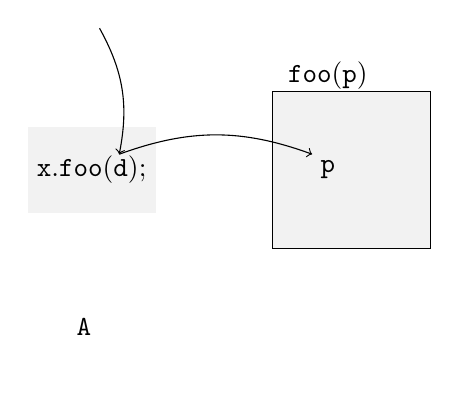
\begin{tikzpicture}
\def\base{1.5}
\def\x{3.0}
\def\xfd{0}
\draw [fill=black!5] (\base + \x + 1.3,1,0) rectangle (\base + \x - 0.7,-1);
\node[minimum size=11mm] (cs) at (\base + \x, 1.2) {$\mathtt{foo(p)}$};
\node[minimum size=11mm, fill=black!5] (cs) at (\base + 0, 0 + \xfd) {$\mathtt{x.foo(d);}$};
\node[minimum size=11mm] (A) at (\base -0.1, \xfd -2) {$\mathtt{A}$};
\node[minimum size=11mm] (p) at (\base + \x, 0) {$\mathtt{p}$};

% edges
\path[->] (\base + 0.1, 1.8) edge [sloped, bend left=20] (\base + 0.35, 0.2 + \xfd); % ... to d
\path[->] (\base + 0.35, 0.2 + \xfd) edge [sloped, bend left=20] (\base + \x - 0.2, 0.2); % d to p 
\end{tikzpicture}
}
        % \caption{Traditional CFL with pre-build call graph}
        \caption{Parameter passing without dispatching}
        \label{fig:approach0}
    \end{subfigure}
    \hspace{-2ex}
    \begin{subfigure}{.32\linewidth}
    \resizebox{0.9\width}{0.9\height}{
        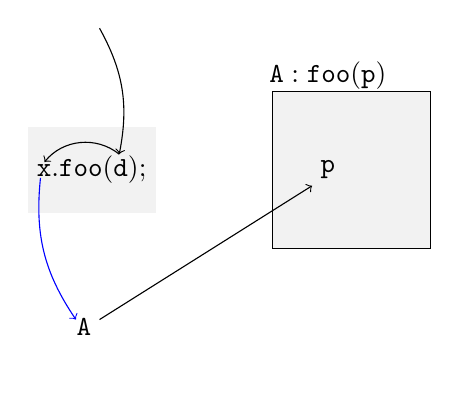
\begin{tikzpicture}
\def\base{1.5}
\def\x{3.0}
\def\xfd{0}
\draw [fill=black!5] (\base + \x + 1.3,1,0) rectangle (\base + \x - 0.7,-1);
\node[minimum size=11mm] (cs) at (\base + \x, 1.2) {$\mathtt{A:foo(p)}$};
\node[minimum size=11mm, fill=black!5] (cs) at (\base + 0, 0 + \xfd) {$\mathtt{x.foo(d);}$};
\node[minimum size=11mm] (A) at (\base -0.1, \xfd -2) {$\mathtt{A}$};
\node[minimum size=11mm] (p) at (\base + \x, 0) {$\mathtt{p}$};

% edges
\path[->] (\base -0.65, -0.1 + \xfd) edge [blue, sloped, bend right=20] (\base -0.2, -1.9 + \xfd); % x to A
\path[->] (\base + 0.1, -1.9 + \xfd) edge [sloped] (\base + \x - 0.2, -0.2); % A to p
\path[->] (\base + 0.1, 1.8) edge [sloped, bend left=20] (\base + 0.35, 0.2 + \xfd); % ... to d
\path[->] (\base + 0.35, 0.2 + \xfd) edge [sloped, bend right=45] (\base -0.6, 0.1 + \xfd); % d to x 
\end{tikzpicture}
}
        % \caption{CFL with build-in call graph building (dispatch on receiver object)}
        \caption{Dispatching at allocation site}
        \label{fig:approach1}
    \end{subfigure}
    \hspace{-2ex}
    \begin{subfigure}{.32\linewidth}
    \resizebox{0.9\width}{0.9\height}{
        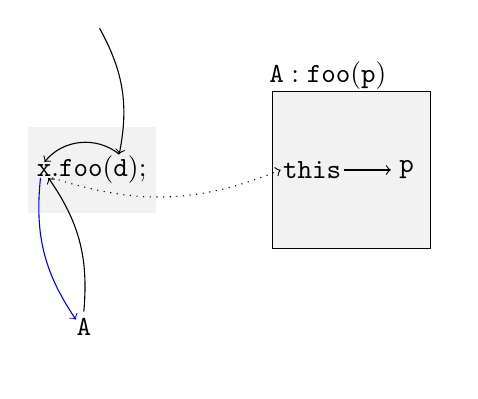
\begin{tikzpicture}
\def\base{1.5}
\def\x{3.0}
\def\xfd{0}
\draw [fill=black!5] (\base + \x + 1.3,1,0) rectangle (\base + \x - 0.7,-1);
\node[minimum size=11mm] (cs) at (\base + \x, 1.2) {$\mathtt{A:foo(p)}$};
\node[minimum size=11mm, fill=black!5] (cs) at (\base + 0, 0 + \xfd) {$\mathtt{x.foo(d);}$};
\node[minimum size=11mm] (A) at (\base -0.1, \xfd -2) {$\mathtt{A}$};
\node[minimum size=11mm] (this) at (\base + \x - 0.2, 0) {$\mathtt{this}$};
\node[minimum size=11mm] (p) at (\base + \x + 1, 0) {$\mathtt{p}$};

% edges
\path[->] (\base -0.65, -0.1 + \xfd) edge [blue, sloped, bend right=20] (\base -0.2, -1.9 + \xfd); % x to A
\path[->] (\base -0.1, -1.8 + \xfd) edge [sloped, bend right=20] (\base -0.55, -0.1 + \xfd); % A to x

%\path[->] (0.1, -2.8) edge [sloped] (3.8, -0.2); % A to p
\path[->] (\base + 0.1, 1.8) edge [sloped, bend left=20] (\base + 0.35, 0.2 + \xfd); % ... to d
\path[->] (\base + 0.35, 0.2 + \xfd) edge [sloped, bend right=45] (\base -0.6, 0.1 + \xfd); % d to x 
\path[->] (\base -0.5, -0.1 + \xfd) edge [dotted, sloped, bend right=20] (\base + \x - 0.6, 0.0); % x to this 
\path[->] (\base + \x + 0.2, 0) edge [sloped] (\base + \x + 0.8, 0.0); % this to p 
\end{tikzpicture}
}
        % \caption{New CFL with build-in call graph building}
        \caption{Dispatching at callsite}
        \label{fig:approach2}
    \end{subfigure}
    \caption{Different ways of handling parameter passing at a virtual call.}
    \label{fig:approach}
\end{figure*}

Below, we illustrate how we address \challenge{1} and \challenge{2} in $L_F$.

\paragraph{\challenge{1} } We address the first challenge, i.e., associating the value flow of arguments with that of receiver variables, by enforcing the value flows from arguments (return values) to their corresponding receiver variables with specially designed \pag edges, i.e., \store[i] and \load[\texttt{ret}], added via \rulename{Call}. According to \rulename{P-Call}, dynamic dispatching values from an argument $a_i$ to a formal parameter $p_i^{m'}$ dependents on $t$ (the dynamic types of the receiver objects), $\texttt{m}$ (the signature of the invoking method), and $i$ (the identifier of the argument it self).   While the later two could be obtained at hand, the receiver objects and the receiver variable $a_0$ could be further apart in the program, separated by a long sequence of method calls (with complex field accesses). 

\Cref{fig:approach} displays three different ways of handling parameter
passing. As illustrated in \Cref{fig:approach0}, the traditional CFL-reachability
formulation directly pass arguments to parameters in callee methods,
which fails to reflect the process of dispatching due to the value flow of arguments
and receiver variables are independent and thus results in a less precise precision
(as stated earlier). The algorithm-assisted dispatching approach
\cite{sridharan2005demand, sridharan2006refinement} in such case initiates an
on-demand points-to
analysis for the receiver variable and once its points-to information is obtained, the dispatching
could be proceeded smoothly. Likewise, our formulation also triggers a $\iflowsto$ process to find
receiver objects before performing dispatching (as illustrated with \textcolor{blue}{blue} edge in \Cref{fig:approach1} and \Cref{fig:approach2}). The difference is that we also need to record the
identifier in $L_F$ stack (reflected by \store[i/\texttt{ret}] in \rulename{Call} and
\rulename{Return}). The method signature is not explicitly encoded into the $L_F$ stack as our
formulation enforces the value flow comes back to the callsite before performing dispatching which
will be discussed shortly. 

\paragraph{\challenge{2} } We address the second challenge (i.e., choosing a
suitable dispatching location) by performing dispatch at callsites. There are
two potential suitable locations for performing dispatching after finding 
receiver objects.
One is dispatching in place (as illustrated in \Cref{fig:approach1}) and
another is performing
dispatching after returning back to the original callsite (\Cref{fig:approach2}). 
Our way of handling is the second one and we use 
\Cref{fig:LFStackChangeAlongValueFlow} for a brief illustration. 
In \Cref{fig:LFStackChangeAlongValueFlow}, the $L_F$-path  from \commentfont{D}
to \texttt{p} is given together with the corresponding $L_F$ stack. Initially, the $L_F$ stack is empty. At callsite \texttt{c3}, our grammar will put $\store[1]$ into $L_F$ stack, indicating that it starts to dispatch argument $d$ to the corresponding parameter, and then trigger a $\iflowsto$ process to find the receiver objects of \texttt{x}. Once we have found that the receiver variable \texttt{x} points to object \commentfont{A}, the grammar (\dispatch) first writes the type
information of the receiver object (via $\typefound[\mathtt{A}]$) to the $L_F$ stack and then
enforce the value flow to return to the callsite via a $\flowsto$ process. Next, the terminal $\indispatch[\mathtt{A}]$
enforce the dispatch to be correct by matching the a right receiver type, i.e., \texttt{A} and finally $\load[1]$ ensure the values are
dispatched to the correct parameter by matching the right identifier.  
The process of finding the right return values for a return variable involves an inverse dispatching procedure as the parameter passing, which is omitted here but still defined in \dispatch. 

\begin{figure*}[htbp]
    \centering
\begin{tabular}{c}
\commentfont{D} 
$ \xrightarrow{\new} \texttt{d}\xrightarrow{\store[1]}\texttt{x}$
$\xrightarrow{\iassign}\texttt{a}
\xrightarrow{\inew}$\commentfont{A}$\xrightarrow{\typefound[\texttt{A}]}$
\commentfont{A}$\xrightarrow{\new} \texttt{a} \xrightarrow{\assign} \texttt{x}\xrightarrow{\indispatch[\texttt{A}]} \texttt{this}^{\texttt{A:foo()}} \xrightarrow{\load[i]}\texttt{p}
$
\end{tabular}

\begin{tikzpicture}[stack/.style={minimum size=5mm, rectangle split, rectangle split parts=#1,draw, anchor=center}]
\node[stack=3] (p0) at (-12, 0) {};

\node[stack=3] (p1) at (-9.5, 0) {
\nodepart{three}1
};

\node[stack=3] (p2) at (-5, 0) {
\nodepart{two}A
\nodepart{three}1
};

\node[stack=3] (p3) at (0, 0) {
\nodepart{three}1
};

\node[stack=3] (p4) at (2, 0) {
};
\end{tikzpicture}
    \caption{An example for illustrating the content of $L_F$ stack changes along the value flow path from \commentfont{D} to \texttt{p}. We use 1 and \texttt{A} to represent $\store[1]$ and $\typefound[\mathtt{A}]$ for brevity. }
    \label{fig:LFStackChangeAlongValueFlow}
\end{figure*}

% When a value is passed to a virtual callsite as an argument, we cannot immediately know which specific method parameter the argument should go to. Instead, we should first query the receiver of this callsite to see which objects it points to, so as to decide where to go according to its type. After that, the grammar will enforce it to return to the callsite. Then, we will be able to know the correct dispatching target according to the type information obtained.

Below, we explain why dispatching in place (\Cref{fig:approach1}) is not feasible.

In the dispatching process, suppose we also encode the information of method signature into $L_F$ stack (i.e., replacing $\store[\texttt{i}]$ and $\load[\texttt{i}]$ with $\store[\texttt{m:i}]$ and $\load[\texttt{m:i}]$ respectively), then when we find the receiver object, we have gathered all the information needed for dispatching. Context-insensitively, one could use 
the following definition of $\dispatch$ ($\idispatch$ should be changed accordingly but omitted here) to replace the ones in \Cref{eqn:newLF} and obtain a new language denoted as $L_{F'}$ for supporting pointer analysis with dynamic dispatching. 
% There seems to be another choice here. 
% In the above process, when we find the receiver object, we have gathered all the information needed for dispatching. One would ask why we must go back to the callsite. It is true if only context-insensitive analysis is considered. For example, we can use \argrec to mark the beginning of searching for a receiver object. After we find the specific object, we need to know which callsite (to be precise, its method signature) is being processed to dispatch correct method according to the type and method signature. We also need to know which parameter is being passed in order to pass the correct parameter after dispatch. This can be solved by adding a set of balanced parentheses with method signature and parameter: When we start looking for receiver object at \argrec, we introduce the method signature of the callsite and the target parameter on the stack. That is, \argrec[m:i]. After finding the specific object, we can match it with, say, \recparm[m:i] to pass the argument to the correct formal parameter, which can be established statically. That is, the previous "entry" edge in \rulename{P-Call} is parsed with \argrec[m:i] \iflowsto \recparm[m:i] rather than a simple \assign edge as before. And the non-terminal \flows in \cref{eqn:callsiteLF} is changed to:
\begin{equation} \scriptsize
\label{eqn:newFlows}
\begin{split} 
\dispatch & \longrightarrow \store[\texttt{m:i}]\ \iflowsto\ \load[\texttt{m:i}]\\
        & \longrightarrow \store[\texttt{m:ret}] \ \flowsto \ \load[\texttt{m:ret}]
\end{split}
\end{equation}
% "exit" edge in \rulename{P-Call} and \iflows in \cref{eqn:callsiteLF} should be changed accordingly but omitted here. The process of this kind of way of handling of parameter passing is illustrated in \cref{fig:approach1}.

However, the context after the parameter passing is different from the traditional
formulation \cite{sridharan2005demand, sridharan2006refinement} which depends on 
a known control-flow by doing so. Consider the following flow path from 
\commentfont{O1} to \texttt{v} (again but this time) expressed by $L_{F'C}$ as \Cref{eq:alterLFPath}:
\begin{equation} \scriptsize
  \centering
\label{eq:alterLFPath}
\begin{tabular}{l} 
\commentfont{O1}$\xrightarrow{\new}
\texttt{o1}\xrightarrow[\hat{\mathtt{c1}}]{\assign}
\texttt{o} \xrightarrow{\store[f]} \texttt{d}
\xrightarrow{\inew}$ 
\commentfont{D} 
$ \xrightarrow{\new} \texttt{d}\xrightarrow{\store[\texttt{foo:1}]}\texttt{x}$\\
\scriptsize
$\xrightarrow[\check{\mathtt{c1}}]{\iassign}\texttt{a}
\xrightarrow{\inew}$\commentfont{A}$\xrightarrow{\load[\texttt{foo:1}]}\texttt{p}
    \xrightarrow{\load[f]} \texttt{v}
$
\end{tabular}
\end{equation}
% For example, if we simply apply \cref{eqn:newFlows}, we will find that although we can find the correct formal parameter for this single parameter passing, the context for \texttt{p} or \texttt{v} after the parameter passing is not as expected. We note the language $L_F$ modified with \cref{sec:newFlows} as $L_{F'}$. The path from \commentfont{O1} to 
% \texttt{v} is expressed by $L_{FC}$ as \cref{eq:LFCPathCGPreciseI} but is expressed by $L_{F'C}$ as \cref{eq:alterLFPath}:
The $L_C$ strings for \texttt{v} in \Cref{eq:LFCPathCGPreciseI} and 
\Cref{eq:alterLFPath} are $\hat{\mathtt{c1}}\hat{\mathtt{c3}}$ and
$\hat{\mathtt{c1}}\check{\mathtt{c1}}$, respectively, resulting in 
inconsistent calling contexts for \texttt{v} (i.e., $[\mathtt{c3}, \mathtt{c1}]$ and \emptyctx ~ respectively) when the parameter passing is completed.
We know that the callsite-sensitivity is modeling call stacks, so $L_{F'C}$ is incorrect
for a callsite-sensitive analysis. Note that attempting to encode context information 
into below-edges in \pag (e.g., replacing $\xrightarrow{\load[\texttt{foo:1}]}$ in
\Cref{eq:alterLFPath} with $\xrightarrow[\hat{\texttt{c1}};\hat{\texttt{c3}}]{\load[\texttt{foo:1}]}$) 
is also infeasible as one method may be invoked under different calling contexts with a same receiver object and statically establishes $L_C$ strings from receiver variables to receiver objects would be another challenge. 

% By returning to the callsite after finding the receiver object, changing the dispatching location to callsite, and together with the following new $L_C$, \challenge{4} can be addressed.

\subsubsection{$L_C$}
\label{subsubsec:newLC}

The grammar for 
$L_C$ given below enforces the pointer analysis to be fully
callsite-sensitive:
% by not only matching method calls and returns as a balanced-parentheses problem but also ensuring contexts to be restored when dispatching:
%\input{languageC.tex}
%{
%\addtolength\abovedisplayskip{-.5ex}
%\addtolength\belowdisplayskip{-.5ex}
\begin{equation}
\label{eqn:callsiteLC}
\footnotesize
    \begin{split}
\textsf{realisable} \longrightarrow \textsf{exit} ~ \textsf{entry} \\
\textsf{exit} \longrightarrow \textsf{exit} ~ \textsf{B} \mid \textsf{exit} \ \check{c} \mid \epsilon \\ 
\textsf{entry} \longrightarrow \textsf{entry} ~ \textsf{B} \mid \textsf{entry} \ \hat{c} \mid \epsilon \\
\textsf{B} \longrightarrow \textsf{B} ~ \textsf{B} \mid \hat{c} ~ \textsf{B} ~ \check{c} \mid \hat{\boxed{c}} ~ R ~ \check{\boxed{c}} \mid \epsilon \\
R \longrightarrow B ~ R \mid R ~ B \mid \check{c} ~ R ~ \hat{c} \mid H\\
H \longrightarrow B ~ H \mid H ~ B \mid \hat{c} ~ H ~ \check{c} \mid \epsilon\\
    \end{split}
\end{equation}
% \begin{equation}
%     \begin{split}
% L_{R} & \longrightarrow S^*\\
% S & \longrightarrow \check{c_i} \mid \hat{c_i} \mid  R \mid \epsilon\\
% R & \longrightarrow \hat{\boxed{c_i}} ~ restore ~ \check{\boxed{c_i}}\\
% \textsf{restore} & \longrightarrow \check{c_i} ~ \textsf{restore} ~ \hat{c_i} \mid 
% \hat{c_i} ~ \textsf{restore} ~ \check{c_i} \\
% & \longrightarrow R ~ \textsf{restore} ~ R \mid \hat{\tau} \mid \check{\tau}
%     \end{split}
% \end{equation}
%}
%\noindent\hspace*{-1ex}
where the set of terminals includes all the below-edge labels in \pag, 
and $\epsilon$ is the standard symbol denoting the empty string. 

$L_C$ is also an extension of the standard formulation for matching method 
calls and returns by solving also context restoring for supporting dynamic 
dispatching. A path $p$ in \pag is said to be \emph{realizable} iff it is an $L_C$-path.
An unrealizable path in \pag characterizes a value flow that enters a method 
on a callsite but leaves the same method on a different callsite. Below, we highlight that how we address \challenge{3} and \challenge{4} in $L_C$ respectively. 

\paragraph{\challenge{3} } We address the third challenge, i.e., ensuring the values of an argument are correctly delivered to the right parameter, by exploiting the balanced matching property of virtual call dispatching. As stated earlier in $L_F$, we require that $\store[\texttt{i/ret}]$ matched by $\load[\texttt{i/ret}]$ and $\typefound[\texttt{t}]$ matched by $\indispatch[\texttt{t}]$. However, these could not guarantee that dispatching is correct as we have chosen to perform dispatching at callsites (\Cref{fig:approach2}).
Consider the following case (with class \texttt{A} and \texttt{D} defined in \Cref{fig:motivatingExample} and \texttt{A} is modified by adding a new method definition ``\lstinline[language=java]!void goo(D s){}!''):
\begin{lstlisting}[language=java, basicstyle=\small, numbers=none]
D d1 = new D(); // D1
D d2 = new D(); // D2
A a = new A(); // A
a.foo(d1); // c1
a.goo(d2); // c2
\end{lstlisting}
We would have the following flow path from \commentfont{D1} to \texttt{s} to be a valid $L_F$-path due to \commentfont{A} is the receiver object of both callsite \texttt{c1} and \texttt{c2}:
\begin{equation} \scriptsize
  \centering
\label{eq:CH3Case1}
\begin{tabular}{l} 
\commentfont{D1}$\xrightarrow{\new}
\texttt{d1}\xrightarrow{\store[1]}
\texttt{a} \xrightarrow{\inew}$ 
\commentfont{A} $\xrightarrow{\typefound[\texttt{A}]}$ \commentfont{A}
$ \xrightarrow{\new} \texttt{a}\xrightarrow{\indispatch[\texttt{A}]} \texttt{this}^{\texttt{goo}}$\\
\scriptsize
$\xrightarrow{\load[1]}\texttt{s}
% \xrightarrow{\inew}$\commentfont{A}$\xrightarrow{\load[\texttt{foo:1}]}\texttt{p}
%     \xrightarrow{\load[f]} \texttt{v}
$
\end{tabular}
\end{equation}
Encoding method signature into $L_F$ stack as $\store[\texttt{m:i}]$ like that in \Cref{subsubsec:newLF} could eliminate such spurious value flow but still fails if we 
replace ``\lstinline{a.goo(d2); // c2}'' with ``\lstinline{a.foo(d2); // c2}'' since 
the method signature this time no longer distinguishes the two callsites in the later case (denoted \textbf{case 2}). 

We address this problem by encoding callsite information into $L_C$ stack. Let $\hat{\boxed{c}}$ marks the beginning of searching for a receiver object, and $\check{\boxed{c}}$ marks the returning to the original callsite. Once the value flow returns back after finding dispatching type and is ready for dispatching, the $L_C$ requires $\hat{\boxed{c}}$ matched by $\check{\boxed{c}}$ and thus enforces the dispatching is performed at the original callsite. 

Let us revisit \textbf{case 2} with below-edges in the value flow path from \commentfont{D1} to \texttt{p} that passes through callsite \texttt{c2} being considered this time:
\begin{equation} \scriptsize
  \centering
\label{eq:CH3Case2}
\begin{tabular}{l} 
\commentfont{D1}$\xrightarrow{\new}
\texttt{d1}\xrightarrow[\hat{\boxed{\texttt{c1}}}]{\store[1]}
\texttt{a} \xrightarrow{\inew}$ 
\commentfont{A} $\xrightarrow{\typefound[\texttt{A}]}$ \commentfont{A}
$ \xrightarrow{\new} \texttt{a}\xrightarrow[\check{\boxed{\texttt{c2}}};\hat{\texttt{c2}}]{\indispatch[\texttt{A}]} \texttt{this}^{\texttt{foo}}$\\
\scriptsize
$\xrightarrow{\load[1]}\texttt{p}
$
\end{tabular}
\end{equation}
Although this path is an $L_F$-path, it is not an $L_C$-path as $\hat{\boxed{\texttt{c1}}}$ could not be matched by $\check{\boxed{\texttt{c2}}}$.

\paragraph{\challenge{4} } 

\begin{theorem} \label{theorem:CSRecoveryPath}
Let $p$ be any $L_{C}$-path, $\bar{p}$ be the inverse of $p$, and $P = \bar{p};p$ be the concatenation of $\bar{p}$ and $p$, then $P$ could be accepted by language $R$ with productions defined in \Cref{eqn:callsiteLC}. 
\end{theorem}
\begin{proof}
By structure induction.
\end{proof}

\begin{corollary} \label{theorem:LFCRecoveryPath}
Let $p$ be any $L_{FC}$-path, $\bar{p}$ be the inverse of $p$, and $P = \bar{p};p$ be the concatenation of $\bar{p}$ and $p$, then $P$ could be formulated as the intersection of limited context-free languages.
\end{corollary}




\begin{lemma} \label{theorem:Rrealizable}
Let $p$ be an $R$-path and $p'$ be the resulting string after removing $\hat{\boxed{c}}$ 
and $\check{\boxed{c}}$ from $R$, then $p' \in L_{C}^{O}$.  
\end{lemma}

\begin{corollary} \label{theorem:LCrealizable}
Let $p$ be an $L_{C}$-path and $p'$ be the resulting string after removing $\hat{\boxed{c}}$ 
and $\check{\boxed{c}}$ from $L_C(p)$, then $p' \in L_{C}^{O}$.  
\end{corollary}


\begin{lemma} \label{theorem:ContextRecovery}
Let $p$ be an $L_{FC}$-path from any object to an argument $a_i$ at callsite \texttt{c}, and $p'$ be a grammar-guided path from the argument to any receiver object and then returning back to the callsite, (a) $L_C^{entry} (p) = L_C^{entry}(p;p')$ if $|L_C^{entry} (p)| \geq |L_C^{exit}(p')|$.  (b) $L_C^{entry} (p)$ is a suffix of $L_C^{entry}(p;p')$ if $|L_C^{entry} (p)| < |L_C^{exit}(p')|$.
In case (b), $L_C^{entry}(p;p')$ is a more precise context presentation of $a_i$. 
\end{lemma}

\begin{theorem} \label{theorem:correctness}
Let $L_{FC}^{O}$ be the traditional formulation \cite{sridharan2005demand, sridharan2006refinement} defined in \Cref{eqn:callsiteLF} and \Cref{eqn:callsiteLC} over $\pag^{O}$ (the \pag constructed by using rules in 
\Cref{fig:manucflpag}) assisted by an oracle for telling where to perform dispatching at a callsite under certain context,
$L_{FC}^N$ be our new formulation defined in \Cref{eqn:newLF} and \Cref{eqn:callsiteLC} over $\pag^N$ (the \pag constructed by using rules in \Cref{fig:newcflpag}),
then a node $v$ is $L_{FC}^{O}$-reachable from $o$ iff $v$ is $L_{FC}^{N}$-reachable from $o$. 
\end{theorem}

, with $L_C(p)$ being derived from \realizable
starting with the production
$\realizable  \rightarrow \exit\ \entry$.
In this case, we write $L_C^{\exit}(p)$ for the prefix
of $L_C(p)$ that is derived by
\exit and 
$L_C^\entry(p)$ for the suffix of
$L_C(p)$  that is derived by
\entry.
  $\tau$ notes the end of searching for a receiver object. $aaa$ ensures the path between $\tau$ and $\check{\boxed{c}}$ is a symmetry of that from $\hat{\boxed{c}}$ to $\tau$, except those already balanced out. In such a way, the context when coming back to the callsite (after $\check{\boxed{c}}$) should be the same as when starting (before $\hat{\boxed{c}}$). Therefore, \challenge{4} is addressed.

Our CFL-reachability formulation
of \kcs{k}, defined by 
$L_{FC}=L_F\cap L_C$, discovers the points-to information in $G$ as follows.
A path $p$ from $O$ to $v$ in $G$ can be identified as a context-sensitive \flowsto relation iff $p$ is both (1) a $\flowsto$ path in $L_F$, where  $O\;\flowsto\; v$, and (2) a realizable path in $L_C$, where 
$\realizable \Longrightarrow^* L_C(p)$, yielding the following
context-sensitive points-to relation:
%{
%\addtolength\abovedisplayskip{-.3ex}
%\addtolength\belowdisplayskip{-.3ex}
\begin{eqnarray}
\label{eq:pt-ctx}
%\hspace*{-1ex}
\begin{tabular}{@{}r@{\ }c@{\ }l@{}}
$(ctx(L_C^\exit(p)),O)$ & $\in$ &
$\pointsto(ctx(L_C^\entry(p)),v)$\\
\end{tabular}
\end{eqnarray}
where
\begin{eqnarray}
\label{eq:pt-ctx}
\begin{tabular}{@{}r@{\ }c@{\ }l@{}}
$ctx(L_C^\entry(p))$ & $\eqdef$ & sequence of unbalanced  $\hat{c}$\,'s in\\&& $L_C^\entry(p)$ with their hats elided;\\
$ctx(L_C^\exit(p))$ & $\eqdef$ & sequence of  unbalanced  $\check{c}$\,'s in\\&&  
$\overline{L_C^\exit(p)}$ with their checks elided.
\end{tabular}
%\hspace*{-3ex}
\end{eqnarray}

Below we explain how our CFL formulation $L_{FC}=L_F\cap L_C$ works
in finding the points-to information with a build-in call graph establishment mechanism by applying it to the example in \cref{fig:motivatingExample}, whose pointer assignment graph is constructed under the rules in \cref{fig:newcflpag}, as shown in \cref{fig:pag1}.

Let us consider $L_F$ first. By applying our new dispatching rule, a parsing for dispatching path is processed whenever some value flows into \texttt{d} at \inline{x.foo(d); // c3} (line~17). There will be two entry paths generated in total:
\begin{equation}
  \centering
\label{eq:ParmPathI}
\begin{tabular}{l} \scriptsize
$\texttt{d}\xrightarrow{\store[1]}\texttt{x}
\xrightarrow{\iassign}\texttt{a}
\xrightarrow{\inew}$\commentfont{A}$\xrightarrow{\typefound[A]}$\commentfont{A}$\xrightarrow{\new}\texttt{a}\xrightarrow{\assign}\texttt{x}$\\\scriptsize
$\xrightarrow{\indispatch[A]}\texttt{this}^\texttt{A:foo()}\xrightarrow{\load[1]}\texttt{p}$
\end{tabular}
\end{equation}
\begin{equation}
  \centering
\label{eq:ParmPathII}
\begin{tabular}{l} \scriptsize
$\texttt{d}\xrightarrow{\store[1]}\texttt{x}
\xrightarrow{\iassign}\texttt{b}
\xrightarrow{\inew}$\commentfont{B}$\xrightarrow{\typefound[B]}$\commentfont{B}$\xrightarrow{\new}\texttt{b}\xrightarrow{\assign}\texttt{x}$\\\scriptsize
$\xrightarrow{\indispatch[B]}\texttt{this}^\texttt{B:foo()}\xrightarrow{\load[1]}\texttt{q}$
\end{tabular}
\end{equation}
Therefore, the case in \cref{eq:LFCPathCGImprecise} is prohibited as no instance of class \texttt{C} flows to \texttt{x}.

Now, let us update the paths described by \cref{eq:LFCPathCGPreciseI} and \cref{eq:LFCPathCGPreciseII} by replacing the entry path from \texttt{d} to \texttt{p} with the one shown in \cref{eq:ParmPathI}, with $L_C$ also taken into consideration:
\begin{equation}
  \centering
\label{eq:newPathI}
\begin{tabular}{l} \scriptsize
\commentfont{O1}$\xrightarrow{\new}
\texttt{o1}\xrightarrow[\hat{\mathtt{c1}}]{\assign}
\texttt{o} \xrightarrow{\storefield{f}} \texttt{d}
\xrightarrow{\inew}$ \commentfont{D} 
$ \xrightarrow{\new} \texttt{d}\xrightarrow[\hat{\boxed{\texttt{c3}}}]{\store[1]}\texttt{x}
\xrightarrow[\check{\texttt{c1}}]{\iassign}\texttt{a}$\\\scriptsize
$\xrightarrow{\inew}$\commentfont{A}$\xrightarrow[\tau]{\typefound[A]}$\commentfont{A}$\xrightarrow{\new}\texttt{a}\xrightarrow[\hat{\texttt{c1}}]{\assign}\texttt{x}\xrightarrow[\check{\boxed{\texttt{c3}}},\hat{\texttt{c3}}]{\indispatch[A]}\texttt{this}^\texttt{A:foo()}$\\\scriptsize
$\xrightarrow{\load[1]}\texttt{p}
    \xrightarrow{\load[f]} \texttt{v}
$
\end{tabular}
\end{equation}
and
\begin{equation}
  \centering
\label{eq:newPathII}
\begin{tabular}{l} \scriptsize
\commentfont{O2}$\xrightarrow{\new}
\texttt{o2}\xrightarrow[\hat{\mathtt{c2}}]{\assign}
\texttt{o} \xrightarrow{\storefield{f}} \texttt{d}
\xrightarrow{\inew}$ \commentfont{D} 
$ \xrightarrow{\new} \texttt{d}\xrightarrow[\hat{\boxed{\texttt{c3}}}]{\store[1]}\texttt{x}
\xrightarrow[\check{\texttt{c1}}]{\iassign}\texttt{a}$\\\scriptsize
$\xrightarrow{\inew}$\commentfont{A}$\xrightarrow[\tau]{\typefound[A]}$\commentfont{A}$\xrightarrow{\new}\texttt{a}\xrightarrow[\hat{\texttt{c1}}]{\assign}\texttt{x}\xrightarrow[\check{\boxed{\texttt{c3}}},\hat{\texttt{c3}}]{\indispatch[A]}\texttt{this}^\texttt{A:foo()}$\\\scriptsize
$\xrightarrow{\load[1]}\texttt{p}
    \xrightarrow{\load[f]} \texttt{v}
$
\end{tabular}
\end{equation}
We can see that \commentfont{O2} are not $L_{FC}$-reachable to \texttt{v} any more due to unbalanced context in \cref{eq:newPathII}, which meet the expectation in \kcs{2}. For the path shown in \cref{eq:newPathI}, context is successfully restored after dispatching, i.e., it is the same ($\hat{\mathtt{c1}}\hat{\mathtt{c3}}$) as the one in the traditional CFL with a pre-build call graph, compared with the one dispatching at allocation site (\cref{eq:alterLFPath}), which fails to do so.

\subsubsection{$L_X$}
\label{subsubsec:newLX}

As discussed in \Cref{subsec:motivation}, the dispatching for receiver variables and normal arguments are handled differently in \kcs{k} which is not reflected by $L_{FC}^{O}$ and our current formulation, i.e., $L_{FC}^{N}$. For receiver objects, they could only be dispatched to target methods that are compatible with their own types. In order to achieve this goal, we must use a stack to record the type information of the current value flow. 

\Cref{fig:adaptedNewcflpag} shows the adapted \pag construction rules with changes being highlighted in \textcolor{blue}{blue}. We also encode the type information by adding symbols such as $\hat{\boxed{t}}$ and  $\check{\boxed{t}}$ to the below-edges of \pag. 

\begin{figure}[htbp]
\begin{center}
\begin{adjustbox}{width=\linewidth}
\begin{tabular}{c}
			\ruledef{
				 \mathtt{x = \mathsf{\mathbf{new}} ~ T} ~ { \mathtt{//~o}} \rulespace t = \typeof(\mathtt{o})
			}{
				\mathtt{o} \xrightarrow[{\color{blue}\hat{\boxed{t}}}]{\new} \mathtt{x} \rulespace
				\mathtt{o} \xrightarrow[\tau]{\typefound[t]} \mathtt{o}
			}
		 \rulename{New} 
		 \quad
			\ruledef{
			    \mathtt{x = y} 
			}{
				\mathtt{y} \xrightarrow{\assign} \mathtt{x}
			}
			\rulename{Assign}
			\\ [5ex]
	 		\ruledef{
            			    \mathtt{x = y.f} 
            			    \rulespace { \color{blue} t :> \typeof(\texttt{y}) }
            			}{
            				\mathtt{y} \xrightarrow[{\color{blue} \check{\boxed{t}}}]{\loadfield{f}} \mathtt{x}
            			}
        
        	 \rulename{Load}
        	 \quad
			\ruledef{
			    \mathtt{x.f = y} 
			    \rulespace { \color{blue} t :> \typeof(\texttt{x}) }
			}{
				\mathtt{y} \xrightarrow[{\color{blue} \hat{\boxed{t}} }]{\storefield{f}} \mathtt{x} 
			}
			 \rulename{Store}
             \\[5ex]
            	\ruledef{
            			    \mathtt{p} ~ \text{is the } ~ i \text{-th parameter of }~ \texttt{m} ~ (i > 0)
            			    \rulespace { \color{blue} t :> \typeof(\texttt{this}^{\texttt{m}}) }
            			}{
            							\mathtt{this}^{\texttt{m}} \xrightarrow[{\color{blue} \check{\boxed{t}}}]{\loadfield{i}} \mathtt{p} 
            			}
        
        	 \rulename{Param}
        	 \\[5ex]
        % 	 \quad
			\ruledef{
		    \mathtt{r} ~ \text{is the return variable of } ~ \texttt{m}
		    \rulespace { \color{blue} t :> \typeof(\texttt{this}^\texttt{m}) }
			}{
				\mathtt{r}  \xrightarrow[{\color{blue} \hat{\boxed{t}}}]{\storefield{ret}} \mathtt{this}^{\texttt{m}}
			}
			 \rulename{Return}
             \\[5ex]
			\ruledef{
			   \mathtt{x = } ~ a_0.\mathtt{m}(a_1,..., a_r) ~ \mathtt{//~ c} 
			 %  \rulespace o \in \cipointsto{a_0} 
			   \rulespace t :> \typeof(a_0)
			   \rulespace m' = \lookup(\texttt{m}, t) 
			}{
			\rulespace \forall \ i \in [{\color{blue} 1}, r]: a_i \xrightarrow[\hat{\boxed{c}} \ {\color{blue} \hat{\boxed{t}}} ]{\storefield{$i$}} a_0
			\rulespace a_0 \xrightarrow[\check{\boxed{c}} \ {\color{blue} \hat{\boxed{t}}}]{\loadfield{$\texttt{ret}$}} \mathtt{x}
			\rulespace {\color{blue}  a_0 \xrightarrow[\hat{\boxed{c}}]{\assign} a_0 }
            \rulespace a_0 \xrightarrow[\check{\boxed{c}};\hat{c} \ {\color{blue} \check{\boxed{t}};\hat{\boxed{t}}} ]{\indispatch[t]} p_0^{m'} 
			}
			\rulename{Call}
		\end{tabular}
	\end{adjustbox}
	\end{center}
	\caption{The adapted PAG construction rules from \Cref{fig:newcflpag} for supporting dynamic dispatching for receiver objects in our new CFL-reachability formulation. The inverse edges are omitted. Changes are highlighted in \textcolor{blue}{blue}.}
	\label{fig:adaptedNewcflpag}
\end{figure}

To record the type information of current value flow, we add an additional 
CFL grammar $L_X$ which is defined below:
\begin{equation}
\label{eqn:callsiteLX}
\footnotesize
    \begin{split}
L_X  & \longrightarrow  \textsf{Exit} ~ \textsf{Entry} \\
\textsf{Exit}  & \longrightarrow \textsf{Exit} ~ \textsf{xbalance} \mid \textsf{Exit} \ \check{\boxed{t}} \mid \epsilon \\ 
\textsf{Entry}  & \longrightarrow \textsf{Entry} ~ \textsf{xbalance} \mid \textsf{Entry} \ \hat{\boxed{t}} \mid \epsilon \\
\textsf{xbalance} & \longrightarrow \textsf{xbalance} ~ \textsf{xbalance} \mid \hat{\boxed{t}} ~ \textsf{xbalance} ~ \check{\boxed{t}} \mid \epsilon
    \end{split}
\end{equation}
With $L_X$, the top element in $L_X$ stack during the computation of pointer analysis always reflects the type information of current value flow. 

Now, let us revisit the two flow paths given in \Cref{eq:LFCPathCGOnFlyI} and \Cref{eq:LFCPathCGOnFlyII}. We rephrase them in new \pag construction rules given in \Cref{fig:adaptedNewcflpag} listed below:
\begin{equation} \tiny
  \centering
\label{eq:newLFCPathCGOnFlyI}
\begin{tabular}{l} 
\commentfont{A}$\xrightarrow[{\color{blue} \hat{\boxed{\texttt{A}}}}]{\new} \cdots \xrightarrow[{\color{blue} \hat{\boxed{\texttt{D}}}}]{\store[f]} \texttt{d}
\xrightarrow[{\color{blue} \check{\boxed{\texttt{D}}}}]{\inew}$ \commentfont{D} 
$ \xrightarrow[{\color{blue} \hat{\boxed{\texttt{D}}}}]{\new} \texttt{d}
\xrightarrow[{\color{blue} \check{\boxed{\texttt{D}}}}]{\load[f]} \texttt{a}
\xrightarrow[\hat{\boxed{\mathtt{c}}}]{\assign} \texttt{a}
\xrightarrow[\check{\boxed{\mathtt{c}}};\hat{\mathtt{c}} \ {\color{blue} \check{\boxed{\texttt{A}}};\hat{\boxed{\texttt{A}}}}]{\indispatch[\texttt{A}]} \mathtt{this}^{\texttt{A:foo()}}$
\end{tabular}
\end{equation}
\begin{equation} \tiny
  \centering
\label{eq:newLFCPathCGOnFlyII}
\begin{tabular}{l} 
\commentfont{B}$\xrightarrow[{\color{blue} \hat{\boxed{\texttt{B}}}}]{\new} \cdots \xrightarrow[{\color{blue} \hat{\boxed{\texttt{D}}}}]{\store[f]} \texttt{d}
\xrightarrow[{\color{blue} \check{\boxed{\texttt{D}}}}]{\inew}$ \commentfont{D} 
$ \xrightarrow[{\color{blue} \hat{\boxed{\texttt{D}}}}]{\new} \texttt{d}
\xrightarrow[{\color{blue} \check{\boxed{\texttt{D}}}}]{\load[f]} \texttt{a}
\xrightarrow[\hat{\boxed{\mathtt{c}}}]{\assign} \texttt{a}
\xrightarrow[\check{\boxed{\mathtt{c}}};\hat{\mathtt{c}} \ {\color{blue} \check{\boxed{\texttt{A}}};\hat{\boxed{\texttt{A}}}}]{\indispatch[\texttt{A}]} \mathtt{this}^{\texttt{A:foo()}}$
\end{tabular}
\end{equation}
The flow path in \Cref{eq:newLFCPathCGOnFlyII} is an invalid $L_X$-path and thus eliminated. 

Below, we show that $L_X$ and $L_F$ can be merged as a single CFL by encoding type information also into $L_F$ stack in an appropriate order.

\Cref{fig:finalNewcflpag} gives the final \pag construction rules. Comparing with \Cref{fig:adaptedNewcflpag}, we could find that type symbols in the below edges have been moved to the above edges. The \typefound[t] edges have 
been removed as the type information they contains have been expressed in $\new[t]$ and $\inew[t]$. Similarly, 
${\color{blue} \check{\boxed{t}};\hat{\boxed{t}}}$ has been directly removed as \indispatch[t] has already contained the type information. 

\begin{figure}[htbp]
\begin{center}
\begin{adjustbox}{width=\linewidth}
\begin{tabular}{c}
			\ruledef{
				 \mathtt{x = \mathsf{\mathbf{new}} ~ T} ~ { \mathtt{//~o}} \rulespace t = \typeof(\mathtt{o})
			}{
				\mathtt{o} \xrightarrow{\new{\color{blue}[\texttt{t}}]} \mathtt{x} 
				% \rulespace
				% \mathtt{o} \xrightarrow[\tau]{\typefound[t]} \mathtt{o}
			}
		 \rulename{New} 
		 \quad
			\ruledef{
			    \mathtt{x = y} 
			}{
				\mathtt{y} \xrightarrow{\assign} \mathtt{x}
			}
			\rulename{Assign}
			\\ [5ex]
	 		\ruledef{
            			    \mathtt{x = y.f} 
            			    \rulespace { \color{blue} t :> \typeof(\texttt{y}) }
            			}{
            				\mathtt{y} \xrightarrow{\load{\color{blue} [\texttt{t}]}[\texttt{f}]} \mathtt{x}
            			}
        
        	 \rulename{Load}
        	 \quad
			\ruledef{
			    \mathtt{x.f = y} 
			    \rulespace { \color{blue} t :> \typeof(\texttt{x}) }
			}{
				\mathtt{y} \xrightarrow{\store[\texttt{f}]{\color{blue} [\texttt{t}]}} \mathtt{x} 
			}
			 \rulename{Store}
             \\[5ex]
            	\ruledef{
            			    \mathtt{p} ~ \text{is the } ~ i \text{-th parameter of }~ \texttt{m}~(i > 0)
            			    \rulespace { \color{blue} t :> \typeof(\texttt{this}^\texttt{m}) }
            			}{
            							\mathtt{this}^{m} \xrightarrow{\load{\color{blue} [t]}[i]} \mathtt{p} 
            			}
        
        	 \rulename{Param}
        	 \\[5ex]
        % 	 \quad
			\ruledef{
		    \mathtt{r} ~ \text{is the return variable of } ~ \texttt{m}
		    \rulespace { \color{blue} t :> \typeof(\texttt{this}^\texttt{m}) }
			}{
				\mathtt{r}  \xrightarrow{\store{\color{blue} [\texttt{ret}]}[t]} \mathtt{this}^{\texttt{m}}
			}
			 \rulename{Return}
             \\[5ex]
			\ruledef{
			   \mathtt{x = } ~ a_0.\mathtt{m}(a_1,..., a_r) ~ \mathtt{//~ c} 
			 %  \rulespace o \in \cipointsto{a_0} 
			   \rulespace t :> \typeof(a_0)
			   \rulespace m' = \lookup(\texttt{m}, t) 
			}{
			\rulespace \forall \ i \in [{\color{blue} 1}, r]: a_i \xrightarrow[\hat{\boxed{c}} ]{\store[i]{\color{blue}[t]}} a_0
			\rulespace a_0 \xrightarrow[\check{\boxed{c}}]{\load{\color{blue}[\texttt{t}}][\texttt{ret}]} \mathtt{x}
			\rulespace {\color{blue}  a_0 \xrightarrow[\hat{\boxed{c}}]{\assign} a_0 }
            \rulespace a_0 \xrightarrow[\check{\boxed{c}};\hat{c} ]{\indispatch[t]} p_0^{m'} 
			}
			\rulename{Call}
		\end{tabular}
	\end{adjustbox}
	\end{center}
	\caption{The final PAG construction rules for our CFL-reachability formulation. The inverse edges are omitted. }
	\label{fig:finalNewcflpag}
\end{figure}

The final $L_F$ grammar is defined in \Cref{eqn:finalNewLF}. In this grammar, we require that $\store[\texttt{f}][t]$
match with $\load[t][\texttt{f}]$, $\store[\texttt{i}][t]$ match with $\load[t][\texttt{i}]$, and $\new[t]$ match with $\indispatch[t]$. 

\begin{equation} \tiny
\label{eqn:finalNewLF}
\begin{split}
\flowsto & \longrightarrow \new[t]~(\flows~|~\indispatch[t])^*\\
\iflowsto & \longrightarrow (\iindispatch[t]~|~\iflows)^*~\inew[t]\\
\flows & \longrightarrow \assign\\&\qquad|~\store[\texttt{f}][t] \ (\iindispatch[t]~|~\iflows)^*\inew[t]~\new[t]~(\flows~|~\indispatch[t])^* \ \load[t][\texttt{f}]\\&\qquad|~\store[i][t] \ (\iindispatch[t]~|~\iflows)^*\inew[t]~\new[t]~(\flows~|~\indispatch[t])^* \ \load[t][i]\\
\iflows & \longrightarrow \iassign\\&\qquad|~\iload[\texttt{f}][t] \ (\iindispatch[t]~|~\iflows)^*\inew[t]~\new[t]~(\flows~|~\indispatch[t])^* \ \istore[t][\texttt{f}]\\&\qquad|~\iloadfield{i}[t] \ (\iindispatch[t]~|~\iflows)^*\inew[t]~\new[t]~(\flows~|~\indispatch[t])^* \ \istore[t][i]\\
\end{split}
\end{equation}

\subsection{Discussion}
\label{subsec:discussion}

